Questo capitolo verifica le ipotesi H1 e H4 della Sezione~\ref{sec:ipotesi}: la capacità di STERA 30M di apprendere regolarità linguistiche che generalizzano a testi mai visti e la qualità dei racconti che genera, confrontata con TinyStories-8M e TinyStories-33M secondo il protocollo del Capitolo~\ref{cap:capitoli/05-metodologia}.

\section{Andamento del pretraining}\label{sec:curve-pretraining-stera30m}

La \autoref{fig:stera30m-pretraining} riporta la perdita sui batch di addestramento, registrata ogni 20 aggiornamenti, la NLL sul campione DEV fisso e il profilo del learning rate.

\begin{figure}[htbp]
\centering
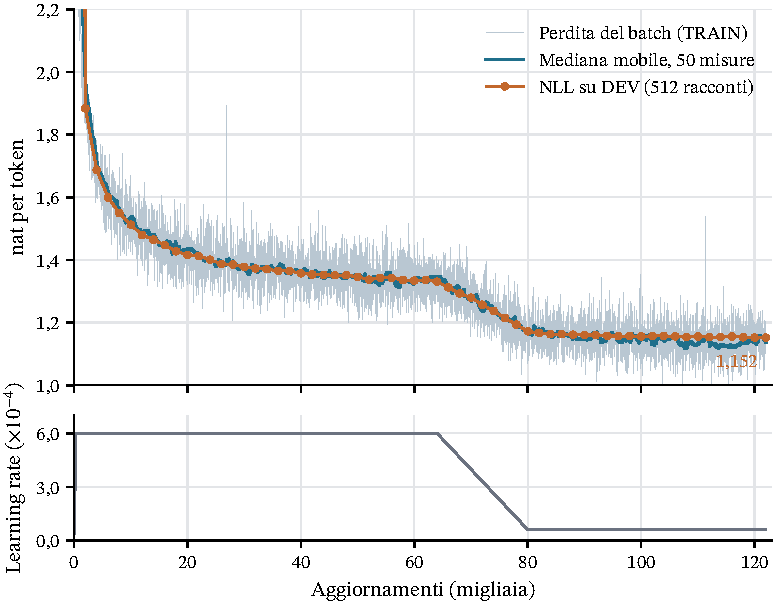
\includegraphics[width=.92\linewidth]{figure/STERA30M/06_pretraining_stera30m.pdf}
\caption{Pretraining di STERA 30M: \num{122000} aggiornamenti e \num{1529514422} token target. In alto, perdita dei batch TRAIN con mediana mobile e NLL sul campione DEV fisso; in basso, learning rate.}
\label{fig:stera30m-pretraining}
\end{figure}

Prima del primo aggiornamento la NLL su DEV è $10{,}928$, prossima a $\ln 50257\approx10{,}82$, il valore di una distribuzione uniforme sul vocabolario. La discesa è rapida nei primi \num{10000} aggiornamenti e prosegue lentamente durante la fase a tasso costante, fino a circa $1{,}33$ al passo \num{64000}. La discesa lineare del learning rate produce un secondo calo marcato, fino a $1{,}172$ al passo \num{80000}. Nella fase finale a tasso ridotto la NLL continua a diminuire lentamente e raggiunge $1{,}152$ (perplessità $3{,}17$) al passo \num{122000}. La perdita su TRAIN e la NLL su DEV restano sovrapposte per tutta la durata dell'addestramento: non si osservano segni di sovradattamento.


\section{Verosimiglianza sui racconti di prova}
\label{sec:risultati-nll}

La Tabella~\ref{tab:nll-3modelli} riporta la NLL dei tre modelli sui 300 racconti TEST, misurata sugli stessi \num{57841} token bersaglio.

\begin{table}[htbp]
\centering
\small
\begin{tabular}{lrrr}
\toprule
Modello & Parametri & NLL & Perplessità \\
\midrule
TinyStories-8M & \num{19702528} & 1,515 & 4,55 \\
\textbf{STERA 30M} & \textbf{\num{30346182}} & \textbf{1,174} & \textbf{3,23} \\
TinyStories-33M & \num{68514048} & 1,324 & 3,76 \\
\bottomrule
\end{tabular}
\caption{NLL media per token sui 300 racconti TEST (\num{57841} token bersaglio) e relativa perplessità.}
\label{tab:nll-3modelli}
\end{table}

STERA 30M ottiene la NLL più bassa. La differenza rispetto a TinyStories-33M è di $-0{,}150$ nat per token, con intervallo bootstrap al 95\% $[-0{,}186;\,-0{,}115]$; rispetto a TinyStories-8M è di $-0{,}341$ nat, con intervallo $[-0{,}365;\,-0{,}319]$. Entrambi gli intervalli escludono lo zero.

Il risultato conferma H1: STERA 30M ha appreso una distribuzione che generalizza a racconti mai visti durante l'addestramento. Il confronto con i riferimenti va però letto con cautela: STERA 30M è stato addestrato sulla stessa versione del corpus da cui provengono i racconti di prova, mentre i dati di addestramento dei checkpoint pubblici non sono documentati con la stessa precisione. Una parte del vantaggio può quindi dipendere dalla corrispondenza fra distribuzione di addestramento e distribuzione di prova, e non solo dal modello.

\section{Qualità dei racconti generati}
\label{sec:risultati-stera30m-tinystories}

\subsection{Quota di racconti corretti}

La Figura~\ref{fig:narrativa-3modelli} e la Tabella~\ref{tab:narrativa-3modelli} riportano l'esito del giudizio cieco sulle 900 continuazioni.

\begin{figure}[htbp]
\centering
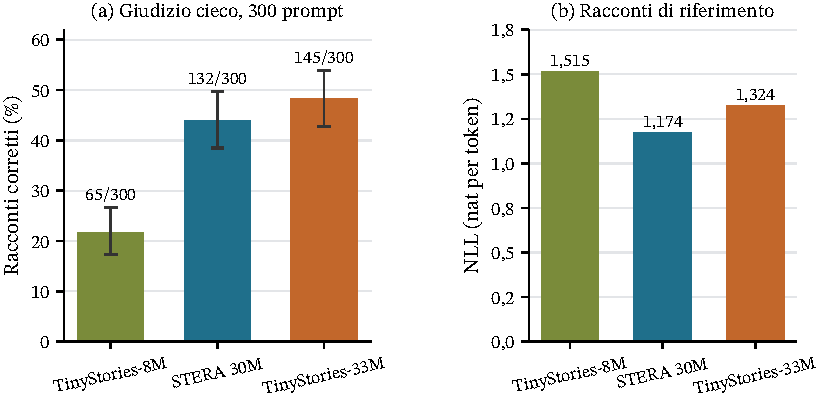
\includegraphics[width=\linewidth]{figure/risultati/narrativa_nll_3modelli.pdf}
\caption{(a) Quota di racconti corretti nel giudizio cieco sui 300 incipit, con intervallo di Wilson al 95\%. (b) NLL sui 300 racconti di riferimento.}
\label{fig:narrativa-3modelli}
\end{figure}

\begin{table}[htbp]
\centering
\small
\begin{tabular}{lrrrrrr}
\toprule
Modello & Corretti & IC 95\% & Grammatica & Coerenza & Trama \\
\midrule
TinyStories-8M & 65/300 (21,7\%) & [17,4; 26,7] & 7,43 & 4,74 & 4,96 \\
\textbf{STERA 30M} & \textbf{132/300 (44,0\%)} & [38,5; 49,7] & 7,67 & 5,26 & 5,37 \\
TinyStories-33M & 145/300 (48,3\%) & [42,7; 54,0] & 7,91 & 5,54 & 5,49 \\
\bottomrule
\end{tabular}
\caption{Racconti corretti con intervallo di Wilson e voti medi (scala 1--10) assegnati dal giudice per grammatica, coerenza e trama.}
\label{tab:narrativa-3modelli}
\end{table}

La gerarchia è netta per la grammatica, che resta alta per tutti i modelli, ed è più marcata per coerenza e trama, le dimensioni che distinguono un racconto corretto da uno che contiene contraddizioni o eventi scollegati. La Figura~\ref{fig:categorie-spn} mostra la distribuzione delle tre categorie: STERA 30M ha una quota di racconti gravemente incoerenti (N) simile a quella di TinyStories-33M, 16 contro 15, e meno della metà di quella di TinyStories-8M, 35.

\begin{figure}[htbp]
\centering
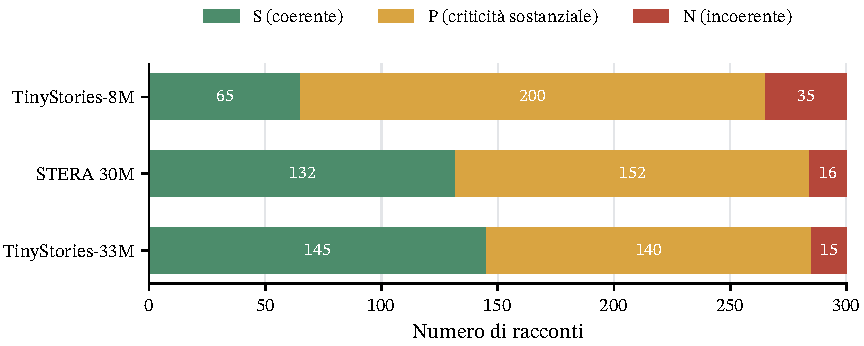
\includegraphics[width=.95\linewidth]{figure/risultati/categorie_spn_3modelli.pdf}
\caption{Distribuzione delle categorie assegnate dal giudice ai 300 racconti di ciascun modello.}
\label{fig:categorie-spn}
\end{figure}

\subsection{Confronti appaiati}

Poiché i tre modelli continuano gli stessi incipit, il confronto più informativo è quello appaiato, incipit per incipit (Tabella~\ref{tab:appaiati-3modelli}).

\begin{table}[htbp]
\centering
\small
\begin{tabularx}{\linewidth}{Xrrrr}
\toprule
Confronto & Differenza & IC 95\% & Solo A / solo B & $p$ (Holm) \\
\midrule
STERA 30M $-$ TinyStories-8M & $+22{,}3$ & $[+15{,}3;\,+29{,}3]$ & 98 / 31 & $<10^{-8}$ \\
STERA 30M $-$ TinyStories-33M & $-4{,}3$ & $[-12{,}0;\,+3{,}7]$ & 66 / 79 & 0,32 \\
TinyStories-33M $-$ TinyStories-8M & $+26{,}7$ & $[+19{,}7;\,+33{,}7]$ & 109 / 29 & $<10^{-10}$ \\
\bottomrule
\end{tabularx}
\caption{Differenze appaiate nella quota di racconti corretti, in punti percentuali. ``Solo A / solo B'' conta gli incipit in cui è corretto solo il primo o solo il secondo modello; il valore $p$ è quello del test esatto di McNemar con correzione di Holm sui tre confronti.}
\label{tab:appaiati-3modelli}
\end{table}

STERA 30M produce racconti corretti molto più spesso di TinyStories-8M: la differenza è di 22 punti percentuali e il test la rende inequivocabile. Rispetto a TinyStories-33M la differenza osservata è di $-4{,}3$ punti e non è statisticamente significativa: sui 145 incipit in cui i due modelli si comportano diversamente, 66 favoriscono STERA 30M e 79 il riferimento. L'intervallo di confidenza, che va da $-12$ a $+4$ punti, non consente tuttavia di affermare che i due modelli siano equivalenti: è compatibile sia con una parità sostanziale sia con uno svantaggio moderato di STERA 30M.

\subsection{Errori ricorrenti}

Le motivazioni del giudice permettono di descrivere gli errori tipici. I racconti classificati P o N dei tre modelli condividono gli stessi difetti, con frequenze diverse: personaggi che cambiano nome o ruolo a metà racconto, oggetti che appartengono prima a un personaggio e poi a un altro, azioni annunciate e mai compiute, morali finali scollegate dagli eventi. Gli errori grammaticali sono rari in tutti e tre i modelli: la difficoltà principale dei modelli di questa scala non è scrivere frasi corrette, ma mantenere stabile lo stato della storia lungo tutto il racconto.

\section{Sintesi}

\begin{itemize}
\item \textbf{H1 è confermata.} La NLL su DEV scende durante tutto l'addestramento e la NLL sui racconti TEST è la più bassa fra i tre modelli confrontati.
\item \textbf{H4 è confermata nei confronti di TinyStories-8M} e \textbf{non è né confermata né smentita nei confronti di TinyStories-33M}. STERA 30M scrive racconti corretti nel 44\% dei casi, il doppio di TinyStories-8M, e con una differenza non significativa rispetto a TinyStories-33M, che ha più del doppio dei parametri memorizzati.
\end{itemize}

Il capitolo successivo verifica le ipotesi H2 e H3, relative al costo di rappresentazione ed esecuzione dei pesi.
